\chapter{Power Law Fit}

\section{Bounded Power Law Fit}

The linear component of the distribution observed in Figure \ref{fig:simulation_statistics} suggests fitting a power law distribution to the simulated sequence of avalanche sizes and areas.

We hypothesize a power law scaling relationship for Toppling Size $S$ and area $A$ of the form:
\[ p(X=x; \tau, x_{max}) = \frac{1}{C_{\tau, x_{max}}} x^{-\tau} \text{ for } x \in \{1, \cdots, x_{max}\}\]
where $x_{max} = x_{max}(L)$ is a cutoff value reflecting the observed decay of the distribution away from power law scaling due to the finite lattice size $L$. 

The shape of the pmf under varying parameter values can be observed in Figure \ref{fig:powerlaw_params}.


\begin{figure}
\begin{center}
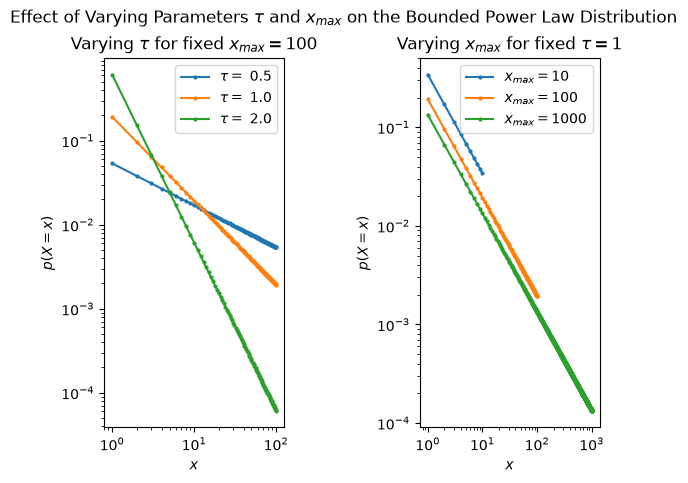
\includegraphics[width=0.80\linewidth]{figures/powerlaw_params.png}
\end{center}
\caption{Visualisation of the bounded power law probability mass function on log-log axes under different parameter combinations. Each point represents a discrete value and corresponding probability mass, with a line connecting sequential points for illustration purposes. The left plot shows the effect of varying $\tau$ while keeping $x_{max}$ constant, which results in changes to the slope and intercept of the connecting line. The right plot shows the effect of varying $x_{max}$ while keeping $\tau$ constant, which results in vertical translation of the connecting line, with different support for $x$. The orange line is identical in both plots, corresponding to parameters $\tau = 1$, $x_{max} = 100$.}
\label{fig:powerlaw_params}
\end{figure} 

To estimate the power law scaling coefficient $\tau$, we apply the method of Maximum Likelihood as justified in Section \ref{sec:stats}. 

Let $\mathbf{x} = (x_1, x_2, \cdots, x_n)$. The likelihood function is:

\begin{align*}
    \mathcal{L}(\mathbf{x}; \tau, x_{max}) &= \prod_{i=1}^n \frac{x_i^{-\tau}}{C_{\tau, x_{max}}} \\
    \log \mathcal{L}(\mathbf{x}; \tau, x_{max}) &= -n \log C_{\tau, x_{max}} -\tau \sum_{i=1}^n \log{x_i} \\
    \intertext{Where $C_{\tau, x_{max}}$ is the normalising constant:}
    C_{\tau, x_{max}} &= \sum_{k=1}^{x_{max}} k^{-\tau}
\end{align*}

To estimate the parameter $\tau$ assuming known $x_{max}$, we compute its Maximum Likelihood Estimate (MLE).
This is the value $\hat{\tau}$ that satisfies:
\[\hat{\tau} = \argmax_{\tau} \mathcal{L}(\mathbf{x}; \tau, x_{max}) = \argmin_{\tau} \left\{- \log \mathcal{L}(\mathbf{x}; \tau, x_{max}) \right\}\]

\textbf{A practical note:} Because the normalising constant $C_{\tau, x_{max}}$ depends on the parameter $\tau$, we cannot find an analytic solution for $\hat{\tau}$ and rely on numerical optimisation techniques.
The numerical optimisation technique used here is the L-BFGS-B algorithm introduced by Byrd et al. (1995) \cite{byrd1995limited} and implemented in the \texttt{scipy} python library. 
Vectorisation is used via \texttt{numpy} arrays to improve the efficiency of the likelihood estimation, which requires computing the log-pmf of each sample point. 
Finally, to prevent numerical underflow when dealing with tiny probabilties of tail events, the \texttt{logsumexp} function from \texttt{scipy} was used; this function provides an underflow-resistant method for calculating an expression of the form $\log \sum_{i} e^{Q_i}$ where $e^{Q_i}$ ranges across a range of scales, which was the case when computing the normalising constants.
These methods were used across all likelihood estimations in this project.

Let $\tau = \tau_s(L), x_{max} = s_{max}(L)$ for modelling the avalanche size, $\tau = \tau_a(L), x_{max} = a_{max}(L)$ for modelling the avalanche area, and $\tau = \tau_d(L), x_{max} = d_{max}(L)$ for modelling the avalanche $L_1$ length.
We first consider a full-data estimation procedure, where we ignore the non-linear distribution tails and fit $\tau$ for each statistic considered and lattice size simulated. Here, we fix $a_{max}(L) = L^2$, $d_{max}(L) = 2L$, and $s_{max}(L) = 10L^2$ as known; this is clearly justified as the theoretical maximum for avalanche area and $L_1$ length, and is a computational adjustment for avalanche size that exceeds any observed avalanche size in the simulated data.

Under the finite size scaling hypothesis discussed in \ref{sec:stats}, we expect that the power law coefficient should be constant for all values of $L$, i.e. we expect $\tau_s(L) = \tau_s$, $\tau_a(L) = \tau_a$, and $\tau_d(L) = \tau_d$.


The estimates obtained are presented in Figure \ref{fig:powerlaw_taus} and Table \ref{tab:powerlaw_taus}. We observe a decreasing trend in the estimated power law coefficients for both avalanche size and avalanche area. However, in Figure \ref{fig:powerlaw_fitted_mle} we see that the tail has a substantial effect on the fit, creating an artificially high estimate for the slope. This effect appears most pronounced at smaller lattice sizes, but is still evident at $L = 100$, suggesting the decrease in $\hat{\tau}$ could be caused by poor fit at the tails.

\begin{figure}
    \centering

    % Left: Figure
    \begin{minipage}[c]{0.48\textwidth}
        \centering
        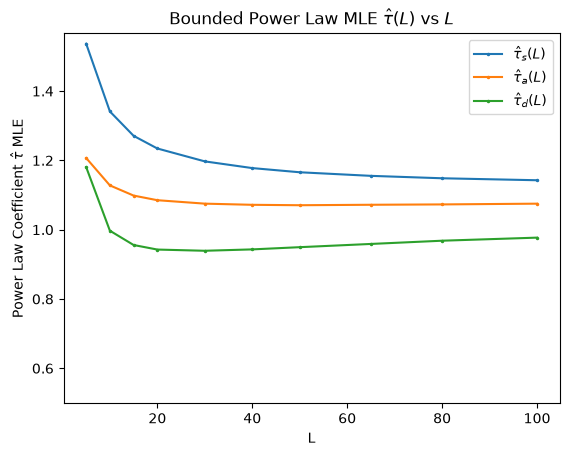
\includegraphics[width=\linewidth]{figures/powerlaw_tau_MLE_vs_L_curve.png}
        \captionof{figure}{Estimates for $\hat{\tau}_s(L), \hat{\tau}_a(L), \hat{\tau}_d(L)$.}
        \label{fig:powerlaw_taus}
    \end{minipage}
    \hfill
    % Right: Table
    \begin{minipage}[c]{0.48\textwidth}
        \centering
        
        \begin{tabular}{|l|l|l|l|}
        \hline
        $L$ & $\hat{\tau}_s(L)$ & $\hat{\tau}_a(L)$ & $\hat{\tau}_d(L)$\\
        \hline
            5 &  1.54 &  1.21 &  1.18 \\
            10 &  1.34 &  1.13 &  1.00 \\
            15 &  1.27 &  1.10 &  0.96 \\
            20 &  1.23 &  1.09 &  0.94 \\
            30 &  1.20 &  1.08 &  0.94 \\
            40 &  1.18 &  1.07 &  0.94 \\
            50 &  1.17 &  1.07 &  0.95 \\
            65 &  1.16 &  1.07 &  0.96 \\
            80 &  1.15 &  1.07 &  0.97 \\
            100 &  1.14 &  1.08 &  0.98 \\
        \hline
        \end{tabular}
        \captionof{table}{Bounded Power Law MLE coefficients $\hat{\tau}$ obtained for varying lattice sizes $L$}
        \label{tab:powerlaw_taus}
    \end{minipage}

\end{figure}

\begin{figure}
\begin{center}
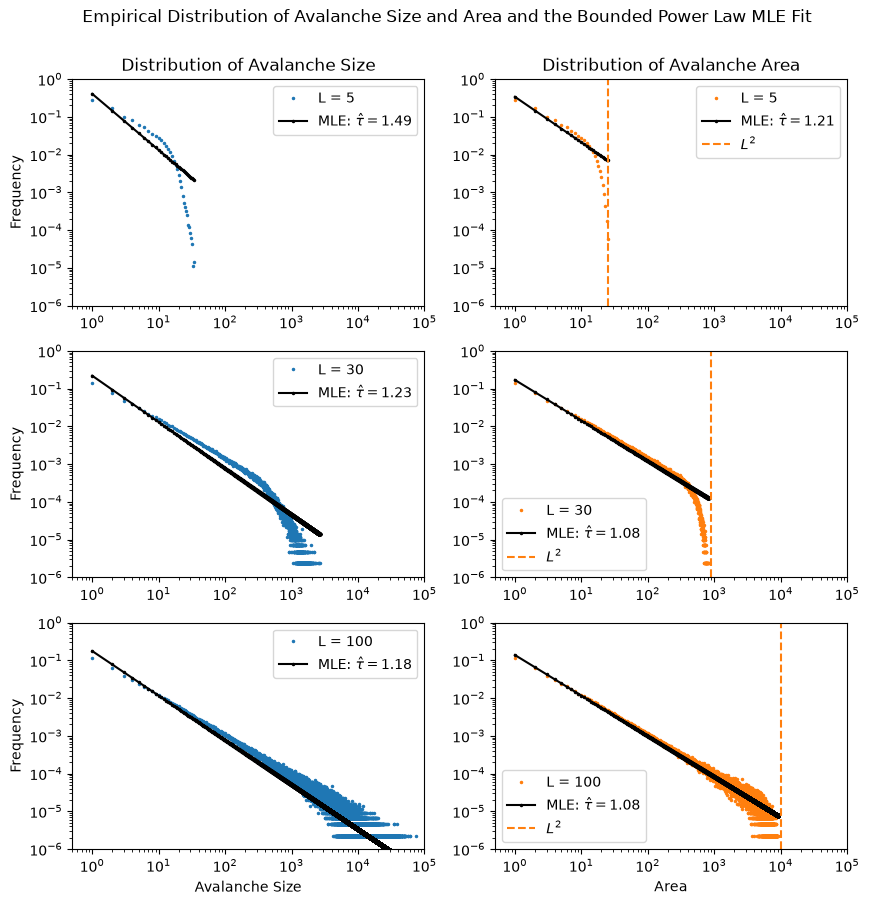
\includegraphics[width=\linewidth]{figures/powerlaw_mle_viz.png}
\end{center}
\caption{Full-data bounded power law MLE fits are skewed down from the true power law coefficient due to the tail decay. Select lattice sizes $L = 5, 30, 100$ are depicted. The fits for all lattice sizes are depicted in Appendix Figure \ref{fig:APPENDIX_powerlaw_mle_viz}. MLEs are drawn as black points with a connecting line drawn for illustration purposes. The left column shows avalanche size, the centre column shows avalanche area, while the right column shows avalanche $L_1$ length. The dashed vertical lines represent the fixed parameter $x_{max}$.}
\label{fig:powerlaw_fitted_mle}
\end{figure} 

\newpage
\section{Manually-truncated Power Law}

As a first correction for the finite lattice effect, we consider restricting $s_{max}, a_{max}, d_{max}$ to include only those topple sizes, areas, and lengths for which linearity is observed in the log-log plot. As we saw in Figure \ref{fig:powerlaw_params}, changing $x_{max}$ should not affect the estimated slope of the distribution.

To avoid manually setting an arbitrary maximum for each value of $L$, here we consider the rule-of-thumb approximation $s_{max}=0.2 L^2, a_{max}= 0.1 L^2, d_{max} = 0.5 L$.
Clearly, there are significant limitations to this approach: the cutoff rule was chosen arbitrarily, and data is significantly limited for lower values of L. However this will help us get a more accurate idea of the power law structure.


The results in Table \ref{tab:powerlaw_trunc_taus} and Figure \ref{fig:powerlaw_trunc_taus} are noticeably lower than the previous estimates in Table \ref{tab:powerlaw_taus}, with an increasing trend rather than decreasing. The fits in Figure \ref{fig:powerlaw_trunc_fitted_mle} are reasonably good for avalanche size and area, however nonlinearity is visible in the avalanche $L_1$ distance plot. This may indicate that the assumed power law scaling is not as well supported from the obtained distribution as it is for size and area.

From these two analyses, it is reasonable that the powerlaw-governed section of the distribution has exponent $\tau_s, \tau_a \approx 1$, which is consistent with the estimate presented in the original 1987 paper by Bak et al. \cite{btw1987intro}. 

\begin{figure}
    \centering

    % Left: Figure
    \begin{minipage}[c]{0.48\textwidth}
        \centering
        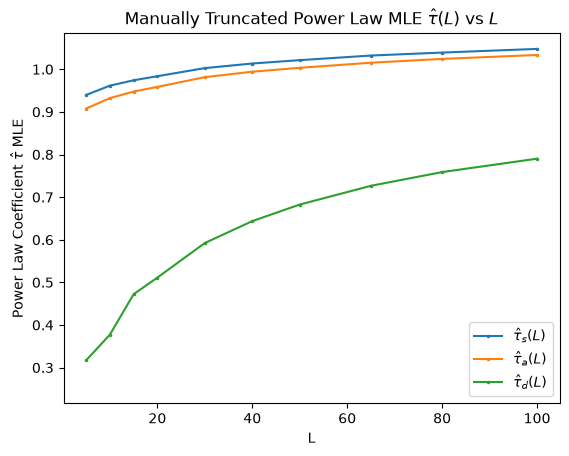
\includegraphics[width=\linewidth]{figures/powerlaw_trunc_taus_taua_plot.png}
        \captionof{figure}{Estimates for $\hat{\tau}_s(L), \hat{\tau}_a(L), \hat{\tau}_d(L)$ under the manual truncation rule $s_{max} = 0.2L^2, a_{max} = 0.1 L^2, d_{max}=0.5L$.}
        \label{fig:powerlaw_trunc_taus}
    \end{minipage}
    \hfill
    % Right: Table
    \begin{minipage}[c]{0.48\textwidth}
        \centering
        \begin{tabular}{|l|l|l|l|}
        \hline
        $L$ & $\hat{\tau}_s(L)$ & $\hat{\tau}_a(L)$ & $\hat{\tau}_d(L)$\\
        \hline
            5 &  0.94 &  0.91 &  0.32 \\
            10 &  0.96 &  0.93 &  0.38 \\
            15 &  0.97 &  0.95 &  0.47 \\
            20 &  0.98 &  0.96 &  0.51 \\
            30 &  1.00 &  0.98 &  0.59 \\
            40 &  1.01 &  0.99 &  0.64 \\
            50 &  1.02 &  1.00 &  0.68 \\
            65 &  1.03 &  1.02 &  0.73 \\
            80 &  1.04 &  1.02 &  0.76 \\
            100 &  1.05 &  1.03 &  0.79 \\
        \hline
        \end{tabular}
        \captionof{table}{MLE power-law slopes obtained for varying lattice sizes $L$ under the manual truncation rule $s_{max} = 0.2L^2, a_{max} = 0.1 L^2, d_{max}=0.5L$}
        \label{tab:powerlaw_trunc_taus}
    \end{minipage}

\end{figure}


\begin{figure}
\begin{center}
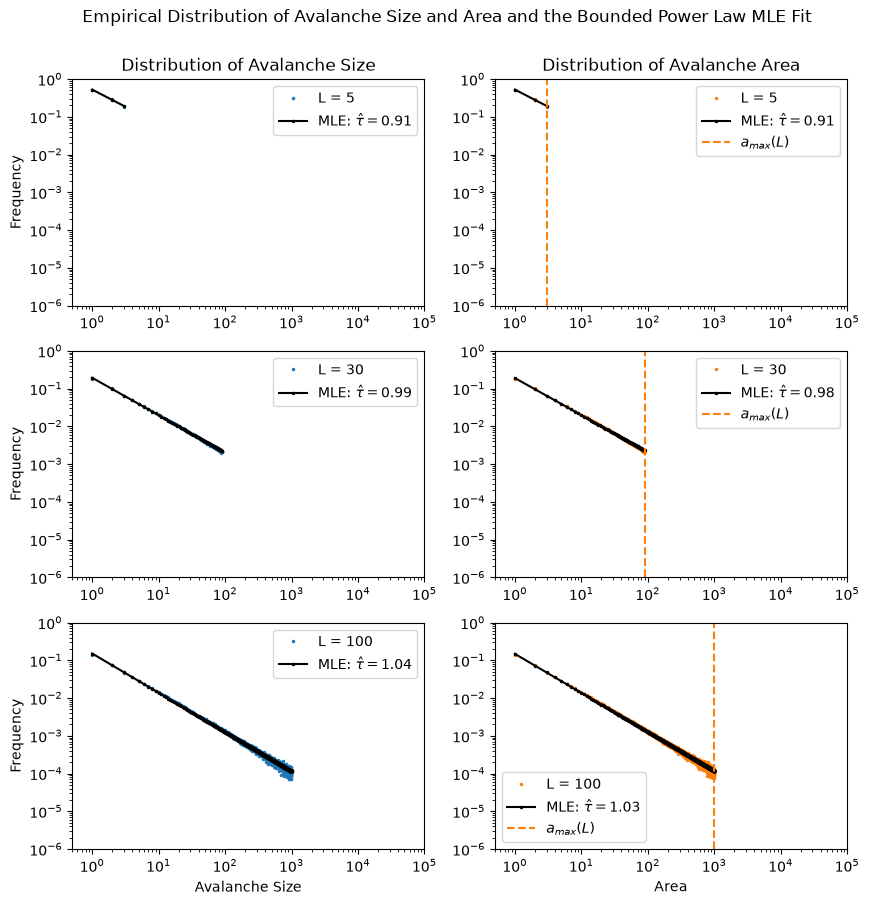
\includegraphics[width=\linewidth]{figures/powerlaw_trunc_mle_viz.png}
\end{center}
\caption{MLE Estimates of the power law scaling coefficient obtained by manually truncating the data tail. Lattice sizes $L = 5, 30, 100$ are depicted - the full data fits are shown in Appendix Figure \ref{fig:APPENDIX_trunc_powerlaw_mle_viz}. MLEs are drawn as black points with a connecting line drawn for illustration purposes. The left column shows avalanche size, the centre column shows avalanche area, and the right column shows avalanche $L_1$ length. The dashed vertical lines on the right show the manual truncation rule bounds $s_{max} = 0.2L^2, a_{max} = 0.1 L^2, d_{max}=0.5L$.}
\label{fig:powerlaw_trunc_fitted_mle}
\end{figure} 

To avoid discarding data, and to model the distribution explicitly, we turn to models that allow for tail decay. We attempt to capture the effect of the finite lattice size $L$ and obtain a more informed approximation to the power law scaling coefficient.